\documentclass[a4paper]{article}

\usepackage{graphicx}
\usepackage{subfig}
\usepackage{multirow}
\usepackage[utf8]{inputenc}

\graphicspath{{figuras/}}

\hyphenation{ve-ri-fi-car FalaBrasil}

\title{Relatório 05}

\author{Pedro Batista (08080002701) - pedro@ufpa.br}

\begin{document}

\maketitle

\section{Influencia de Polos e Zeros no LGR}

O sistema que iremos adicionar polos e zeros para analisar sua influência é:
\begin{equation}
G(s)=\frac{2}{s(s+1)}
\label{eq:r51}
\end{equation}
o ganho pode ser defino garantindo a estabilidade em todo $k>0$. Como
mostrado na Figura~\ref{fig:r51a}.

\begin{figure}[h]
   \subfloat[LGR para o sistema da Equação
      ~\ref{eq:r51}.]{\label{fig:r51a}\includegraphics[width=0.5\textwidth]{r51a}}
   \subfloat[LGR para o sistema da Equação
      ~\ref{eq:r51} adicionado de um polo em $-2$.]{\label{fig:r51b}\includegraphics[width=0.5\textwidth]{r51b}}\\
   \subfloat[LGR para o sistema da Equação
      ~\ref{eq:r51} adicionado de um zero em $-2$.]{\label{fig:r51c}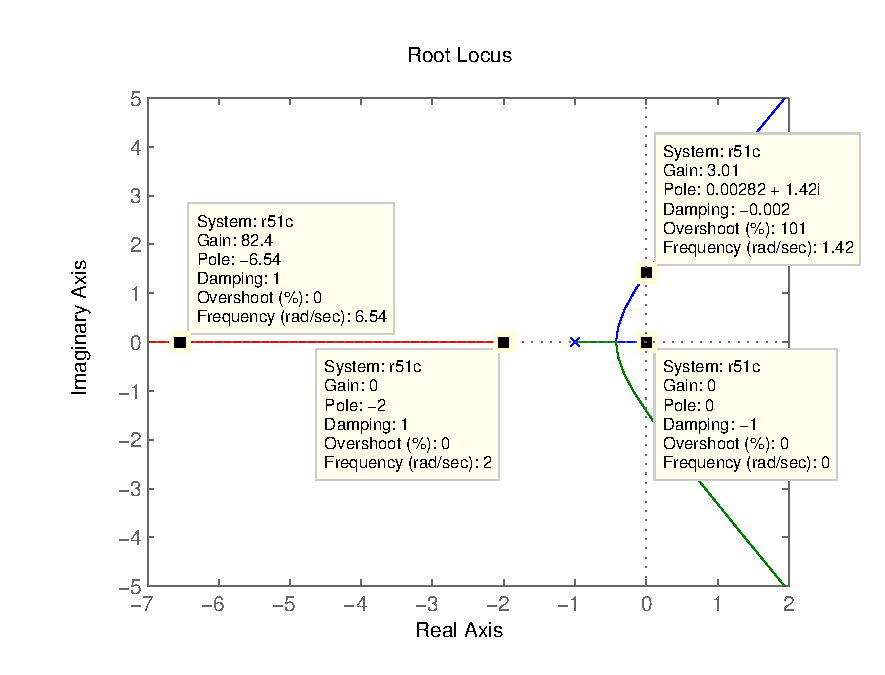
\includegraphics[width=0.5\textwidth]{r51c}}
   \caption{Estudo da influencia de polos e zeros no LGR do sistema.}
   \label{fig:r51}
\end{figure}

\subsection{Influencia de Polos}
A Figura~\ref{fig:r51b} mostra o LGR do sistema da Equação~\ref{eq:r51} com a adição
de um zero em $-2$. Nesta podemos verificar que o ganho ainda é definido para
$k>0$, porém podemos verificar que o sistema ficou mais estável, pois o LGR
ficou mais afastado do semi plano direito.

\subsection{Influencia de Zeros}
É mostrado na Figura~\ref{fig:r51c} o sistema da Equação~\ref{eq:r51}
adicionado de um zero em $-2$, nesse caso tornamos o sistema mais
instável, o ganho que garante a estabilidade no sistema,
está no intervalo $0\leq k \leq 3$.

\section{Observação do LGR de Alguns Sistemas}
Para o sistema da Equação~\ref{eq:r521}, iremos adicionar um zero
em $-3$ e depois um polo em $-1$. O LGR desses três sistemas é mostrado
na Figura~\ref{fig:r521}. Como esperado a Figura~\ref{fig:r52b} mostra
um sistema mais estável que a da Figura~\ref{fig:r52a} gerado pelo novo
zero, já a Figura~\ref{fig:r52c}
mostra o sistema mais instável devido ao novo polo.

\begin{equation}
   G(s)=\frac{1}{s^2+1.2s+1}
   \label{eq:r521}
\end{equation}

\begin{figure}[h]
   \subfloat[LGR para o sistema da Equação
      ~\ref{eq:r521}.]{\label{fig:r52a}\includegraphics[width=0.5\textwidth]{r52a}}
   \subfloat[LGR para o sistema da Equação
      ~\ref{eq:r521} adicionado de um polo em $-1$.]{\label{fig:r52b}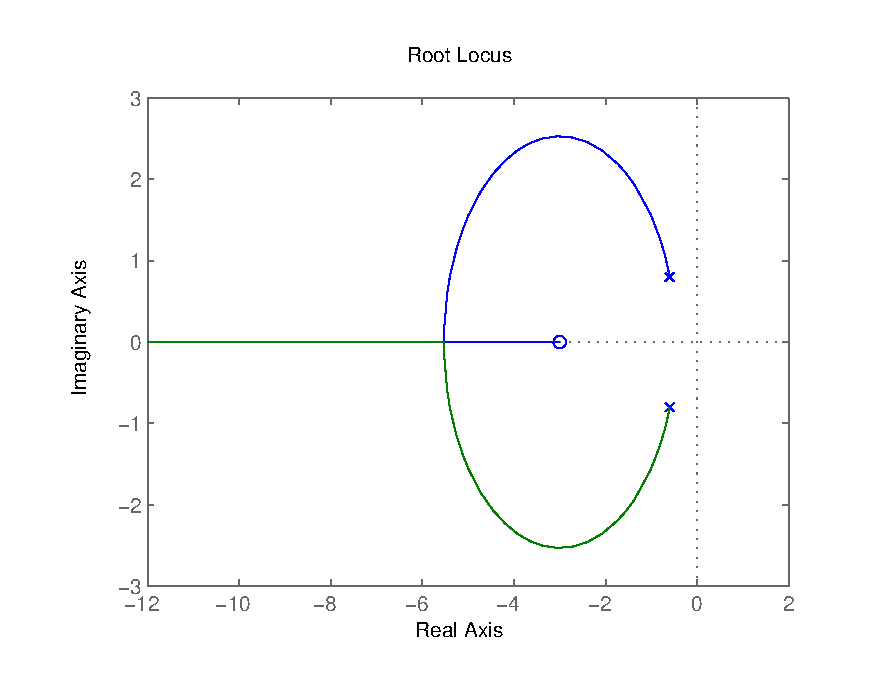
\includegraphics[width=0.5\textwidth]{r52b}}\\
   \subfloat[LGR para o sistema da Equação
      ~\ref{eq:r521} adicionado de um zero em $-3$.]{\label{fig:r52c}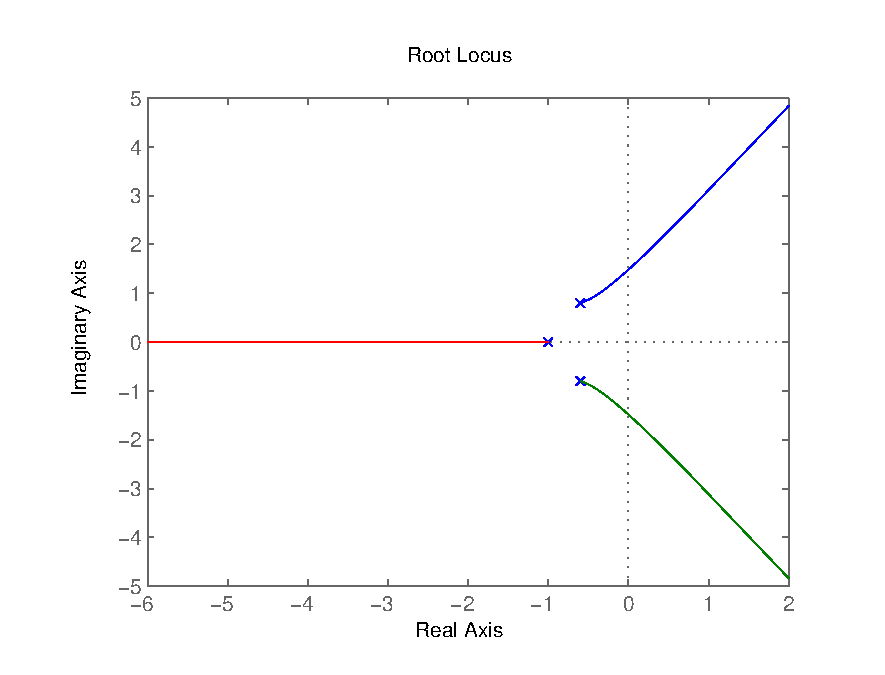
\includegraphics[width=0.5\textwidth]{r52c}}
   \caption{Estudo da influencia de polos e zeros no LGR do sistema.}
   \label{fig:r521}
\end{figure}

O sistema da Equação~\ref{eq:r522} também será analisado, comparando-o com o
da Equação~\ref{eq:r523} no qual afastamos um zero, e
movemos o polo da origem para $-4$. Podemos observar que os dois sistemas
ficaram bastante parecidos, porém o para o da Equação~\ref{eq:r523} quando
o um polo e zero se aproximaram, o sistema passou a ocupar uma maior
área do SPE, tornado-o mais estável.

\begin{equation}
   G(s)=\frac{(s+2)(s+4)}{s(s+1)(s+3)}
   \label{eq:r522}
\end{equation}

\begin{equation}
   G(s)=\frac{(s+2)(s+5)}{(s+4)(s+1)(s+3)}
   \label{eq:r523}
\end{equation}

\begin{figure}[h]
   \subfloat[LGR para o sistema da Equação
      ~\ref{eq:r522}.]{\label{fig:r52d}\includegraphics[width=0.5\textwidth]{r52d}}
   \subfloat[LGR para o sistema da Equação
      ~\ref{eq:r523}.]{\label{fig:r52e}\includegraphics[width=0.5\textwidth]{r52e}}
   \caption{Estudo do LGR de diferentes sistemas.}
   \label{fig:r522}
\end{figure}

\section{Estudo da Adição do Ganho}

\subsection{Sistema de Primeira Ordem}
Para o sistema da Equação~\ref{eq:r53}, desejamos um tempo de reposta igual a $3$
segundos. De acordo com a tabela fornecida no Manual a Equação~\ref{eq:manual_tab1},
podemos definir a posição do polo desejado (igual a $-1$, e o LGR é mostrado na
Figura~\ref{fig:r53_lgr}), e então dar o ganho para o sistema,
o resultado é simulado e mostrado na Figura~\ref{fig:r53_sim}, onde
podemos observar que o tempo foi obedecido.

\begin{equation}
   G(s)=\frac{2}{(s+0.1)}
   \label{eq:r53}
\end{equation}

\begin{equation}
   T_s=\frac{-3}{R}
   \label{eq:manual_tab1}
\end{equation}

\begin{figure}[h]
   \subfloat[LGR para o sistema da Equação
      ~\ref{eq:r53}.]{\label{fig:r53_lgr}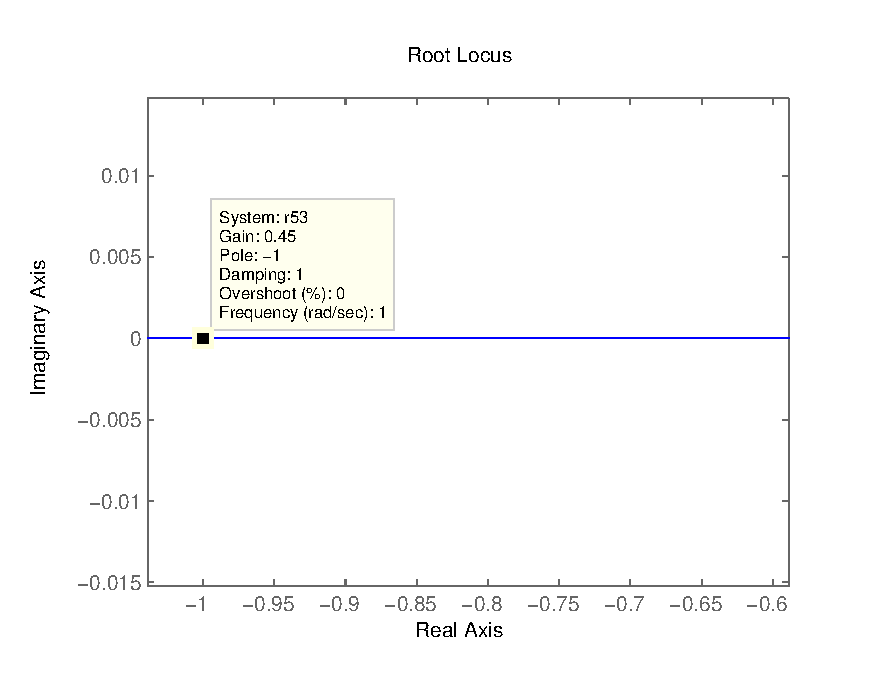
\includegraphics[width=0.5\textwidth]{r53}}
   \subfloat[Simulação para o sistema da Equação~\ref{eq:r53} com a adição de
      um ganho de $0.45$.]{\label{fig:r53_sim}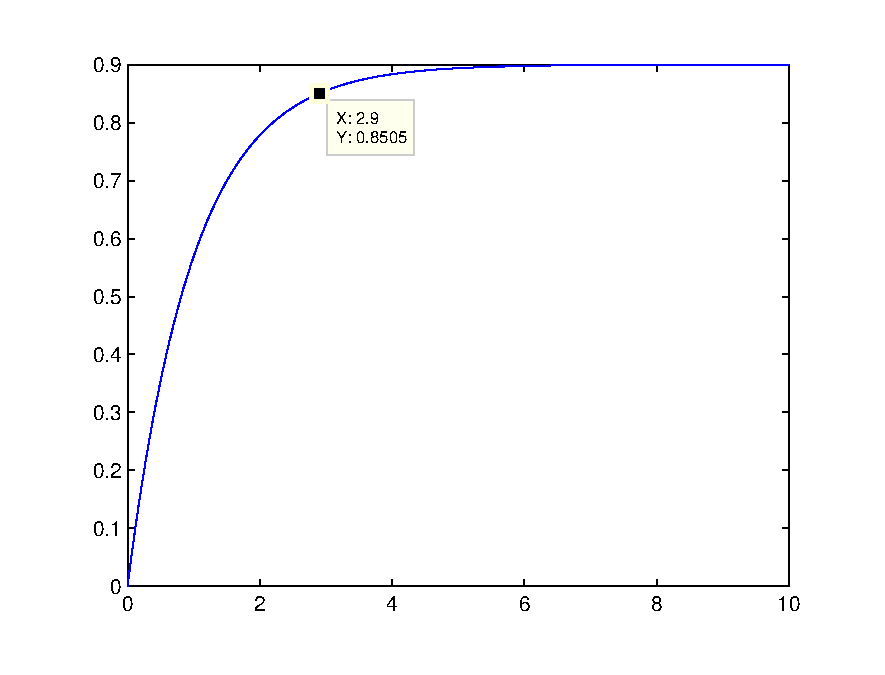
\includegraphics[width=0.5\textwidth]{r53_sim}}
   \caption{Estudo do ganho para que o sistema da Equação~\ref{eq:r53} tenha $T_s=3s$.}
   \label{fig:r53}
\end{figure}

\subsection{Sistema de Primeira Ordem}
Para o sistema da Equação~\ref{eq:r54}, desejamos um sobre-sinal máximo igual a $0.05$.
De acordo com a tabela fornecida no Manual a Equação~\ref{eq:manual_tab2},
podemos definir o valor do $\xi$ desejado (igual a $0.69$, e o LGR é mostrado na
Figura~\ref{fig:r54_lgr}), e então dar o ganho para o sistema,
o resultado é simulado e mostrado na Figura~\ref{fig:r54_sim}, onde
podemos observar que o máximo sobre-sinal de $0.05$ foi obedecido.

\begin{equation}
   G(s)=\frac{2}{s(s+1)}
   \label{eq:r54}
\end{equation}

\begin{equation}
   \xi=\sqrt{\frac{\ln^2(M_p)}{\ln^2(M_p)+\pi^2}}
   \label{eq:manual_tab2}
\end{equation}

\begin{figure}[h]
   \subfloat[LGR para o sistema da Equação
      ~\ref{eq:r54}.]{\label{fig:r54_lgr}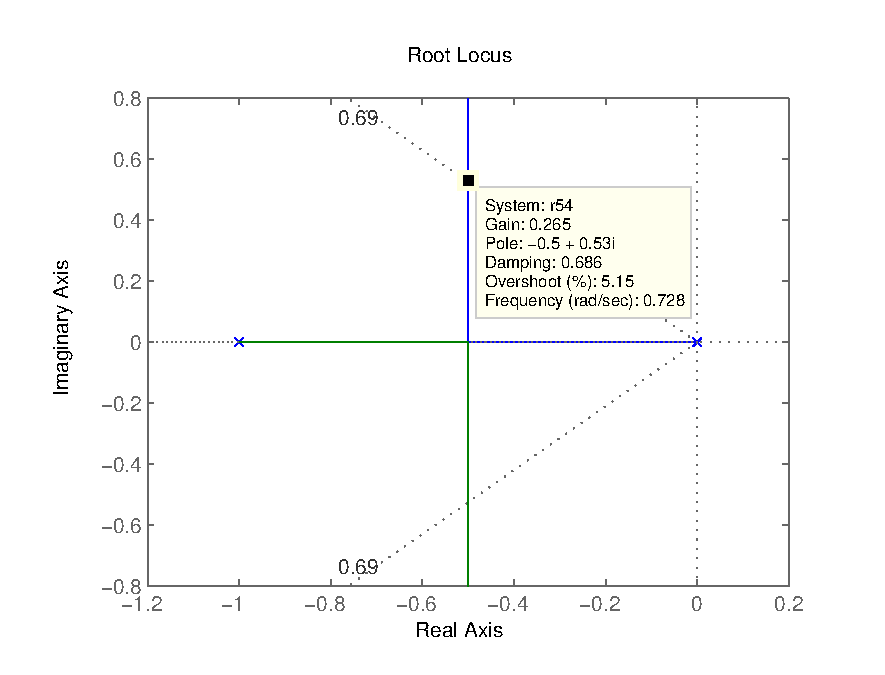
\includegraphics[width=0.5\textwidth]{r54}}
   \subfloat[Simulação para o sistema da Equação~\ref{eq:r53} com a adição de
      um ganho de $0.263$.]{\label{fig:r54_sim}\includegraphics[width=0.5\textwidth]{r54_sim}}
  \caption{Estudo do ganho para que o sistema da Equação~\ref{eq:r54} tenha $M_p=0.05$.}
   \label{fig:r54}
\end{figure}

\bibliographystyle{plain}
\bibliography{bib.bib} 
\end{document}
